\documentclass[12pt, letterpaper]{article}
\usepackage[T1,T2A]{fontenc}
\usepackage[russian]{babel}
\usepackage[utf8]{inputenc}
\usepackage{amsmath}
\DeclareMathOperator\erf{erf}
\usepackage{listings}
\usepackage{xcolor, graphicx}
\usepackage{float}
\usepackage{tikz}
\usepackage{hyperref}
\hypersetup{
    colorlinks=true,
    linkcolor=cyan,
    filecolor=magenta,      
    urlcolor=blue,
    pdfpagemode=FullScreen,
    }

\title{Отчёт по лабораторной работе №22 по курсу “Языки и методы программирования”}
\author{Ибрагимов Далгат Магомедалиевич}
\begin{document}
\maketitle
\begin{description}
\item\textbf{Студент группы:} \underline{М80-108Б-22 Ибрагимов Далгат Магомедалиевич, № по списку 9}    
\item\textbf{Контакты e-mail:} \underline{doly2004e@yandex.ru}
\item\textbf{Работа выполнена:} \underline{«30» апреля 2023 г.}
\item\textbf{Входной контроль знаний с оценкой:} \underline{5}
\item\textbf{Преподаватель:} \underline{асп. каф. 806 Сахарин Никита Александрович}
\item\textbf{Отчет сдан} \underline{«27» мая 2023 г.}, \textbf{итоговая оценка:}\underline{5}
\item\textbf{Подпись преподавателя:} \underline{\hspace{3cm}}
\end{description}
\newpage
\section{Тема}
Издательская система \TeX{}.
\section{Цель работы}
Получить навыки оформления документов в издательской системе \LaTeX{}.
\section{Задание}
Оформить отчёт об изучении \LaTeX{} в издательской системе \LaTeX{}.
\section{Оборудование}
\begin{description}
\item\textbf{Процессор:} AMD RYZEN 5 5600H (12) 3.600GHz
\item\textbf{ОП:} 32 GiB 3200 MHz LPDDR4
\item\textbf{HDD:} 512 Gb
\item\textbf{Монитор:} 1920x1080 240Hz
\end{description}
\section{Программное обеспечение}
\begin{description}
\item\textbf{Операционная система семейства:} Microsoft Windows 11 Pro
\item\textbf{Интерпретатор команд:} pdflatex
\item\textbf{Текстовый редактор:} Visual Studio Code версия 1.73.0
\end{description}
\section{Идея, метод, алгоритм решения задачи}
Прочитать документацию \LaTeX{} и переписать отчет с Markdown на \LaTeX{}. tex-файл скомпилировать с помощью утилиты pdflatex.
\section{Сценарий выполнения работы}
Продемонстрируем широкий функционал \LaTeX{} на следующих примерах.
\subsection{Пример формул}
\[\cos (2\alpha) = \cos^2 \alpha - \sin^2 \alpha = 2\cos\alpha - 1 = 1 - 2\sin\alpha\]
\[C=
\begin{pmatrix}
5 & 2 & 3\\
3 & 5 & 7
\end{pmatrix}\]
\[
\lim\limits_{x \to \infty} \exp(-x) = 0
\] \\
$\mathcal{L}(\theta) = 0.1 \|\theta\|^2 + \frac{1}{N}\sum\limits_{i=1}^N \max(0, 1 - y_i f(x_i, \theta))$ \\
$f(x, \theta) = x_1 \theta_1 + x_2 \theta_2 + \theta_3$ \\
\begin{figure}[h]
\centering
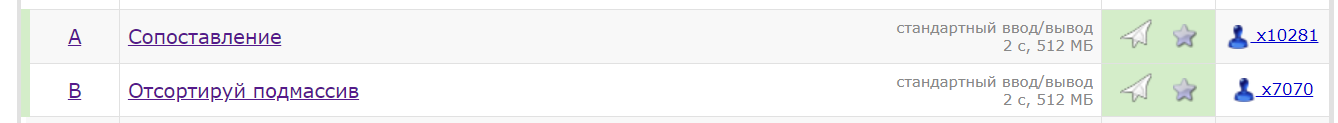
\includegraphics[width=0.9\linewidth]{pic1.png}
\caption{Это подпись к картинкам}
\label{fig:mpr}
\end{figure}
\section{Распечатка протокола}
\begin{lstlisting}[breaklines]
    This is pdfTeX, Version 3.141592653-2.6-1.40.22 (TeX Live 2022/dev/Debian) (preloaded format=pdflatex)
    restricted \write18 enabled.
    entering extended mode
\end{lstlisting}  
\section{Дневник отладки}
\begin{tabular}{|c|p{1cm}|p{1.5cm}|c|p{2.5cm}|p{2cm}|p{2.25cm}|}
    \hline
    № & Лаб. или дом. & Дата & Время & Событие & Действие по исправлению & Примечание\\
    \hline
    1 & Дом. & 4.04.23 & 14:00 & Выполнение лабораторной работы & - & -\\
    \hline
\end{tabular}
\section{Замечания автора по существу работы}
Контест Educational Codeforces Round 147 (Rated for Div. 2) \\
\href{https://codeforces.com/contest/1821/submission/202878443}{1821A - решена на контесте} \\
\href{https://codeforces.com/contest/1821/submission/207354318}{1821B - решена на дорешивании} \\
\section{Выводы}
Были получены навыки оформления докладов в издательской системе \LaTeX{}. Эта система продемонстрировала свою удобность для меня и в дальнейшем будет использована вместо MS Word для оформления курсовых работ по различным предметам. \\
\flushright \textbf{Подпись студента:} \underline{\hspace{3cm}}
\end{document}